%; whizzy chapter -dvi
% -initex iniptex -latex platex -format platex -bibtex jbibtex -fmt fmt
% 以上 whizzytex を使用する場合の設定。

%     Tokyo Debian Meeting resources
%     Copyright (C) 2012 Junichi Uekawa
%     Copyright (C) 2012 Nobuhiro Iwamatsu

%     This program is free software; you can redistribute it and/or modify
%     it under the terms of the GNU General Public License as published by
%     the Free Software Foundation; either version 2 of the License, or
%     (at your option) any later version.

%     This program is distributed in the hope that it will be useful,
%     but WITHOUT ANY WARRANTY; without even the implied warranty of
%     MERCHANTABILITY or FITNESS FOR A PARTICULAR PURPOSE.  See the
%     GNU General Public License for more details.

%     You should have received a copy of the GNU General Public License
%     along with this program; if not, write to the Free Software
%     Foundation, Inc., 51 Franklin St, Fifth Floor, Boston, MA  02110-1301 USA

%  preview (shell-command (concat "evince " (replace-regexp-in-string "tex$" "pdf"(buffer-file-name)) "&"))
% 画像ファイルを処理するためにはebbを利用してboundingboxを作成。
%(shell-command "cd image201205; ebb *.png")

%%ここからヘッダ開始。

\documentclass[mingoth,a4paper]{jsarticle}
\usepackage{monthlyreport}

% 日付を定義する、毎月変わります。
\newcommand{\debmtgyear}{2012}
\newcommand{\debmtgmonth}{8}
\newcommand{\debmtgdate}{18}
% (+ (* (- 2012 2005) 12) 8 -1) started from zero
\newcommand{\debmtgnumber}{91}

\begin{document}

\begin{titlepage}
\thispagestyle{empty}
% タイトルページ:編集必要な部分は最初のマクロに飛ばすこと

\vspace*{-2cm}
第\debmtgnumber{}回 東京エリア Debian 勉強会資料\\
\hspace*{-2cm}
\includegraphics[width=210mm]{image201003/debsen.eps}\\
\hfill{}\debmtgyear{}年\debmtgmonth{}月\debmtgdate{}日

% ここはアップデートすること
% 全角文字にしないとフォントのサイズが合わないので注意
% TODO(uekawa): なんでそうなるのか確認
\rotatebox{10}{\fontsize{32}{32} {\gt 特集: Debconf Report}}\\
\rotatebox{10}{\fontsize{32}{32} {\gt 特集: 月刊Debhelper}}\\

\vspace*{-2cm}
\hfill{}
\includegraphics[height=6cm]{image200502/openlogo-nd.eps}
\end{titlepage}

% Title should be in Japanese text so that we can use it as lint for PDF shiori.
\dancersection{はじめに}{上川 純一}

\begin{multicols}{2}
 

 今月のDebian勉強会へようこそ。これからDebianの世界にあしを踏み入れると
 いう方も、すでにどっぷりとつかっているという方も、月に一回Debianについ
 て語りませんか?

 Debian勉強会の目的は下記です。

 \begin{itemize}
 \item \underline{Debian Developer} (開発者)の育成。
 \item 日本語での「\underline{開発に関する情報}」を整理してまとめ、アップデートする。
 \item \underline{場}の提供。
 \begin{itemize}
  \item 普段ばらばらな場所にいる人々が face-to-face で出会える場を提供
	する。
  \item Debian のためになることを語る場を提供する。
  \item Debianについて語る場を提供する。
 \end{itemize}
 \end{itemize}		

 Debianの勉強会ということで究極的には参加者全員がDebian Packageをがりがり
 と作るスーパーハッカーになった姿を妄想しています。情報の共有・活用を通し
 て Debianの今後の能動的な展開への土台として、「場」としての空間を提供す
 るのが目的です。

\end{multicols}

\newpage

\begin{minipage}[b]{0.2\hsize}
 \definecolor{titleback}{gray}{0.9}
 \colorbox{titleback}{\rotatebox{90}{\fontsize{80}{80} {\gt デビアン勉強会} }}
\end{minipage}
\begin{minipage}[b]{0.8\hsize}
\hrule
\vspace{2mm}
\hrule
\begin{multicols}{2}
\tableofcontents
\end{multicols}
\vspace{2mm}
\hrule
\end{minipage}

\dancersection{事前課題}{上川 純一}

今回の事前課題は以下です:
\begin{enumerate}
 \item Debian 19 周年にちなんで思うことを教えてください。
\end{enumerate}
この課題に対して提出いただいた内容は以下です。
\begin{multicols}{2}
{\small
%; whizzy-master ../debianmeetingresume201208.tex
% $B0J>e$N@_Dj$r$7$F$$$k$?$a!"$3$N%U%!%$%k$G(B M-x whizzytex $B$9$k$H!"(Bwhizzytex$B$,MxMQ$G$-$^$9!#(B
%

\begin{prework}{ $BF|HfLn(B $B7<(B }

19$B<~G/$K$A$J$s$G!"$H$$$&$3$H$G$b$J$$$,!"(B
$B:#G/$O(B Haskell $B$N%i%$%V%i%j$r8x3+$9$kM=Dj$J$N$G!"(B
$B<+J,$G%Q%C%1!<%8%s%0$7$F%a%s%F%J$K$J$j$?$$!#(B
$B$"$H(B Debian Haskell $B%A!<%`$K$b;22C$7$F$$$-$?$$!#(B

\end{prework}

\begin{prework}{ $B$J$+$*$1$$$9$1(B }

$BJQ$o$i$:;H$$B3$1$^$9!#(B
$B$G!"$A$g$C$H$:$D!"(BContribute$B$7$F$$$3$&$H;W$C$F$^$9!#(B
\end{prework}

\begin{prework}{ $BLnEg!!5.1Q(B }

$BJzIi!'(B
$B!V2f$,$"$"(BDebian$B$N!ANO!J$j$g$/(B)$B$O$"$"$"$"@$3&$$$$$$%$%A%$%$%$%$%$%$(B
 $B%$!*!*!*!*!W$H$+8@$($k$HAGE($+$b(B...$B!J!A(B $B$NItJ,$OE,Ev$K(B...)
 
$B$A$g$C$H$0$i$$B>$N?M$,$d$C$?;v$,$J$$$3$H(B1$B$D$G$b(BDebian$B%M%?$G=PMh$?$i$$$$$J(B...$B!VL>>u$7$,$?$$2?$+$N%O!<%I%&%'%"!W$G(BDebian$BF0$+$7$F$_$k$H$+$+$J(B...

\end{prework}

\begin{prework}{ $B%-%?%O%i(B }

$B=tHL$NET9g$GGQ;_$5$l$F$7$^$C$?!"(B
$B2q<R$N(Bdebian$B%5!<%P$rI|3h$5$;$?$$$G$9$M!#(B

\end{prework}

\begin{prework}{ dictoss($B?yK\!!E5=<(B) }

kfreebsd$B$r;H$C$F3Z$7$_$J$,$i!"(Bdeb$B$7$F$$$-$^$9!#(B
\end{prework}

\begin{prework}{ $B@P0f0lIW(B }

DebConf$B$rF|K\$G3+:E$G$-$k$J$i$P!"@'Hs<B8=$5$;$?$$!#(B
\end{prework}

}
\end{multicols}

\dancersection{最近のDebian関連のミーティング報告}{上川 純一}
\subsection{東京エリアDebian勉強会90回目報告}

% (query-replace-regexp "<.*?>" "")
% (query-replace-regexp "^[	 ]\+" "")

東京エリアDebian勉強会。
先週の土曜日は第90回東京エリアDebian勉強会でした。
ニカラグア開催のDebconfが先週あり、先月は大統一Debian勉強会で京都大学にみんな集まった、ということで若干息切れ気味の開催でした。

事前課題はDebconfのビデオをみての感想でした。個人的にはARMの64ビット関連の話題が気になるところ。
MacBookAirにインストールする話題を上川がしました。rEFItとかgptsyncとか知らない人は知らない話題がたくさん。

%-------------------------------------------------------------------------------
\dancersection{Debian Conference 2012参加報告}{岩松 信洋}
%-------------------------------------------------------------------------------

\label{sec:debconfreportsummary}
\index{Debconf2012}
\index{Debconf}

\subsection{Debconfとは}

2012年度の Debconf は 7月8日から7月14日まで、ニカラグアのマナグアで行われました。
日本からは、安井 卓、大岩 達也、矢吹 幸治、山根 秀樹、岩松 信洋が参加しました。

\subsubsection{Debconfの歴史・経緯}

Debian Conference \url{http://debconf12.debconf.org/} は Debian 
の開発者たちが一同に介するイベントです。通常顔をあわせることのないメンバー
たちが一同に介し友好を深め、技術的な議論を戦わせます。過去の開催履歴を見
てみると\tbref{tab:debconflist}のようになります。

\begin{table}[H]
\caption{歴代のDebconf参加者推移}
\label{tab:debconflist}
 \begin{center}
 {\footnotesize
 \begin{tabular}{|c|c|c|r|}
 \hline
 年 & 名前 & 場所 & 参加人数 \\
 \hline
 2000 & debconf 0 &フランス ボルドー & \\
 2001 & debconf 1 &フランス ボルドー & \\
 2002 & debconf 2 &カナダ トロント & 90名 \\
 2003 & debconf 3 &ノルウェー オスロ & 140名 \\
 2004 & debconf 4 &ブラジル ポルトアレグレ &  150名 \\
 2005 & debconf 5 &フィンランド ヘルシンキ & 200名 \\
 2006 & debconf 6 &メキシコ オアスタペック & 300名 \\
 2007 & debconf 7 &英国スコットランド エジンバラ & 約400名 \\
 2008 & debconf 8 &アルゼンチン マルデルプラタ & 約200名 \\               
 2009 & debconf 9 &スペイン エクストラマドゥーラ & 約250名 \\
 2010 & debconf 10 &アメリカ ニューヨーク & 約400名 \\
 2011 & debconf 11 &ボスニア バニャルカ & 約450名 \\
 2012 & debconf 12 &ニカラグア マナグア & 約180名 \\
 \hline
 \end{tabular}
 }
 \end{center}
\end{table}

\subsection{ニカラグア/マナグア}

\subsubsection{行き方}
日本からの行く場合、米国のマイアミかヒューストンからの入国が一番楽
なようです。他の国からは、コスタリカのサンホセやパナマ、アトランタ
から入国できます。
開催施設へはマナグアの空港から約20分ほどタクシーに乗る必要があります。
バスなどもありますが、地元の人の利用者が多いのと治安が悪いためあまり
使わないほうがよいとのこと。
今回ホテルのタクシーに送迎してもらいましたが、地元のタクシーの場合は
10ドルほどの料金がかかります。

\begin{figure}[ht]
\begin{center}
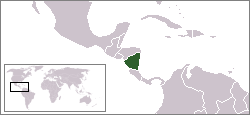
\includegraphics[width=0.8\hsize]{image201208/debconf12_LocationNicaragua.png}
\caption{ニカラグア/マナグアの位置}
\end{center}
\end{figure}
%http://wikitravel.org/ja/%E3%83%95%E3%82%A1%E3%82%A4%E3%83%AB:LocationNicaragua.png

\subsubsection{会場}

\begin{wrapfigure}{r}{11cm}
  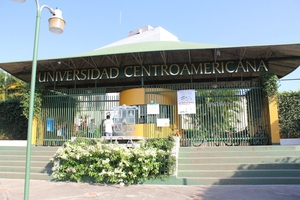
\includegraphics[width=5cm]{image201208/debconf12_mainentry.jpg}
\end{wrapfigure}

2012年度のDebconfの会場はマナグアにある大学「UCA(Universidad Centroamericana」の施設の一部を借りて
行われました。宿泊は会場から5分ほど歩いた場所にあるホテル「Hotel Seminole」で行いました。
以下に会場を紹介します。
\\

\begin{itemize}
  \item Aula Magna Auditorium: メイン用。400人ほど入ることができます。\\
	\begin{minipage}{0.4\hsize}
	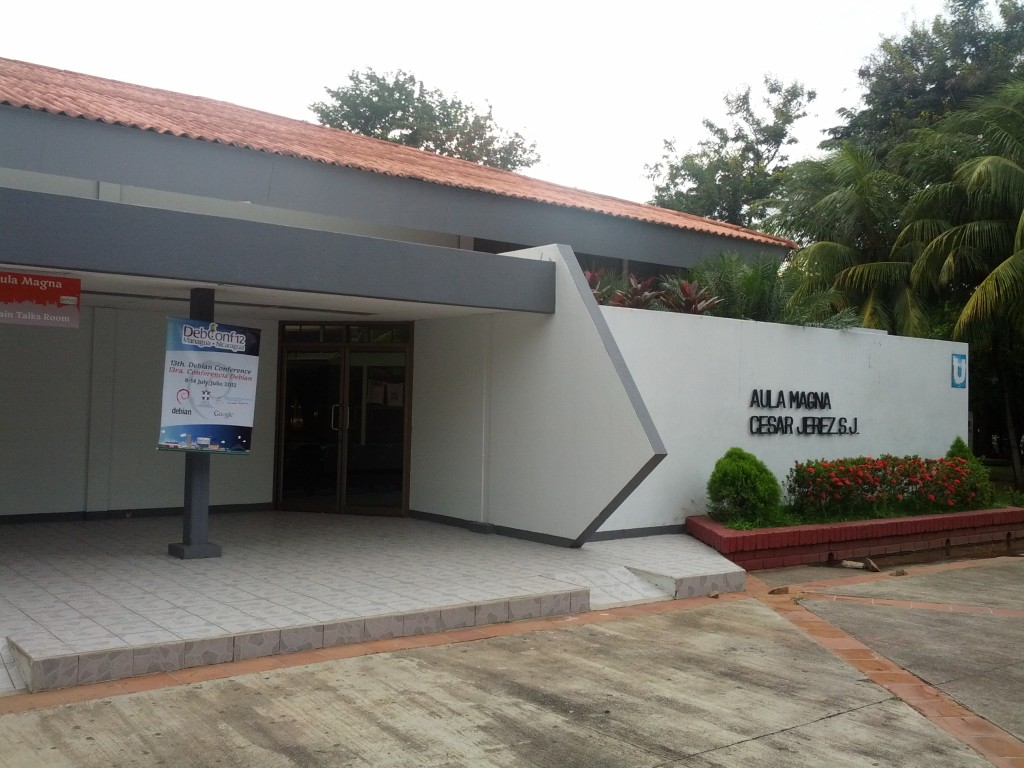
\includegraphics[width=0.8\hsize]{image201208/debconf12_maintalk01.jpg}
        \end{minipage}
        \begin{minipage}{0.4\hsize}
        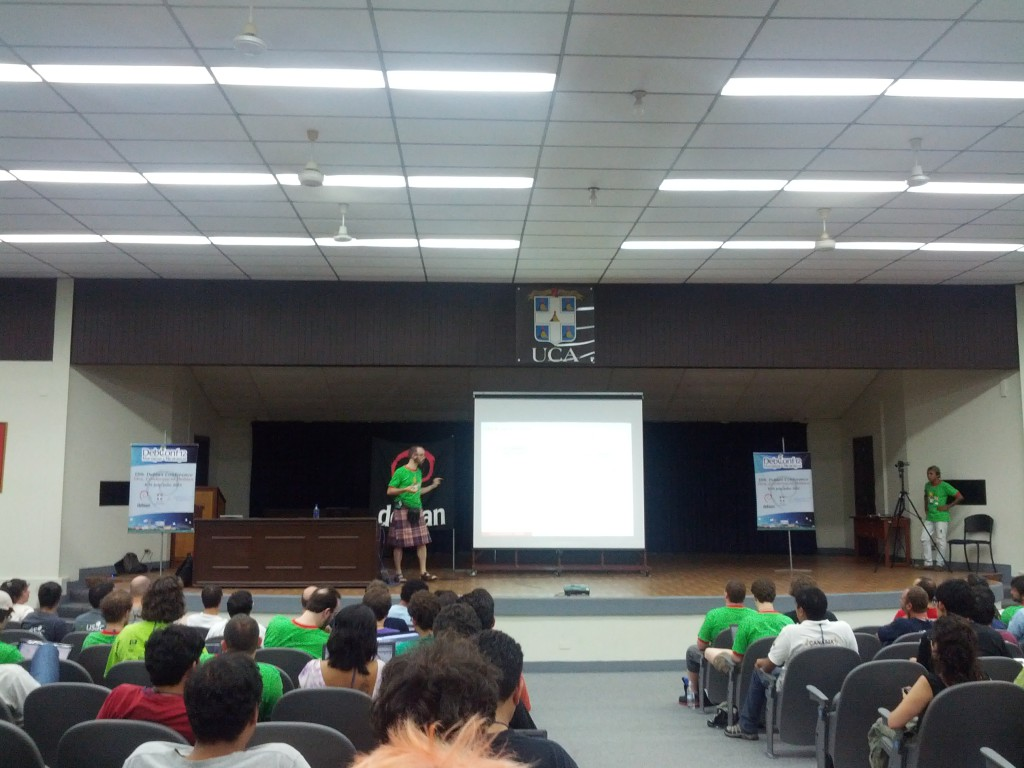
\includegraphics[width=0.8\hsize]{image201208/debconf12_maintalk02.jpg}
	\end{minipage}

  \item Roberto Teran Auditorium: サブ会場。50人ほど入ることができます。\\
        \begin{minipage}{0.4\hsize}
        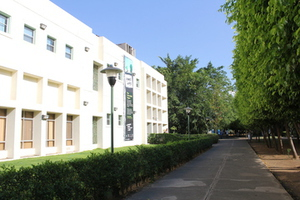
\includegraphics[width=0.8\hsize]{image201208/debconf12_2ndtalkroom01.jpg}
	\end{minipage}
        \begin{minipage}{0.4\hsize}
        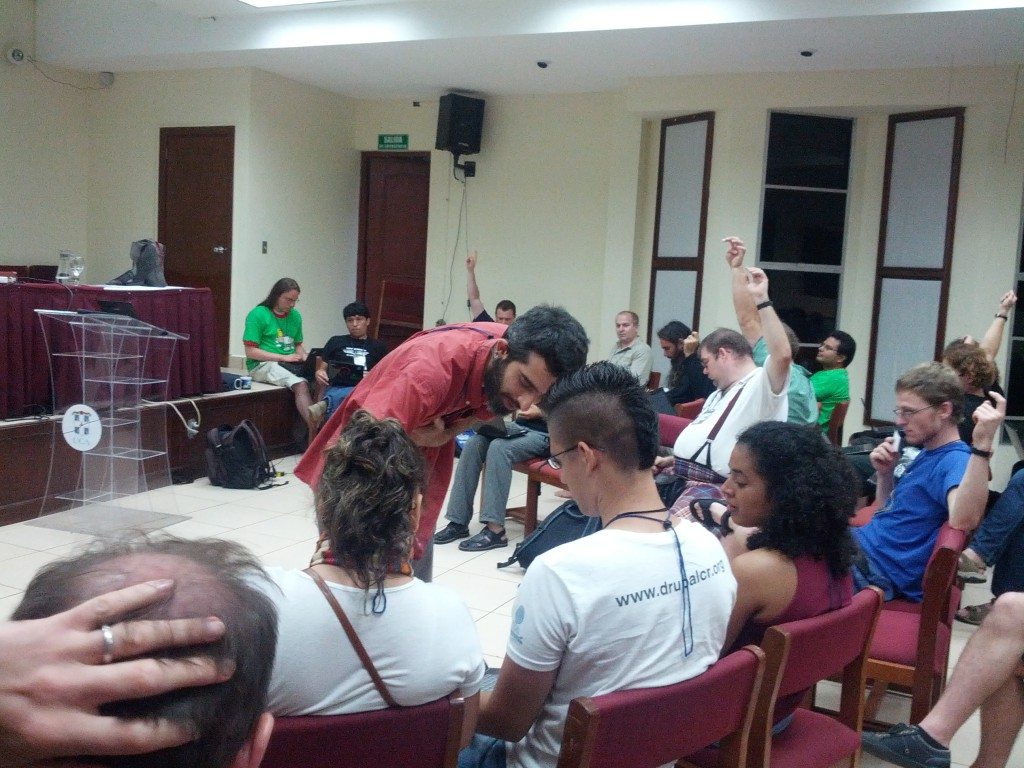
\includegraphics[width=0.8\hsize]{image201208/debconf12_2ndtalkroom02.jpg}
	\end{minipage}

  \item Hacklab: Hacklab はハック専用の部屋です。\\
	\begin{minipage}{0.4\hsize}
	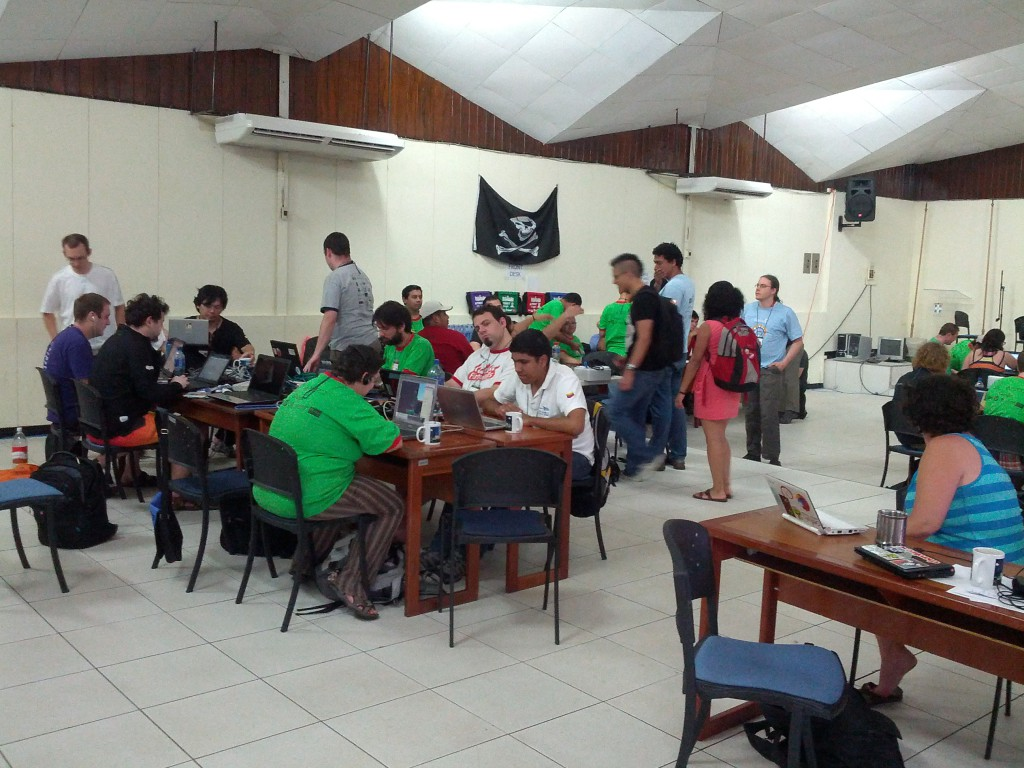
\includegraphics[width=0.8\hsize]{image201208/debconf12_hacklab01.jpg}
	\end{minipage}
        \begin{minipage}{0.4\hsize}
        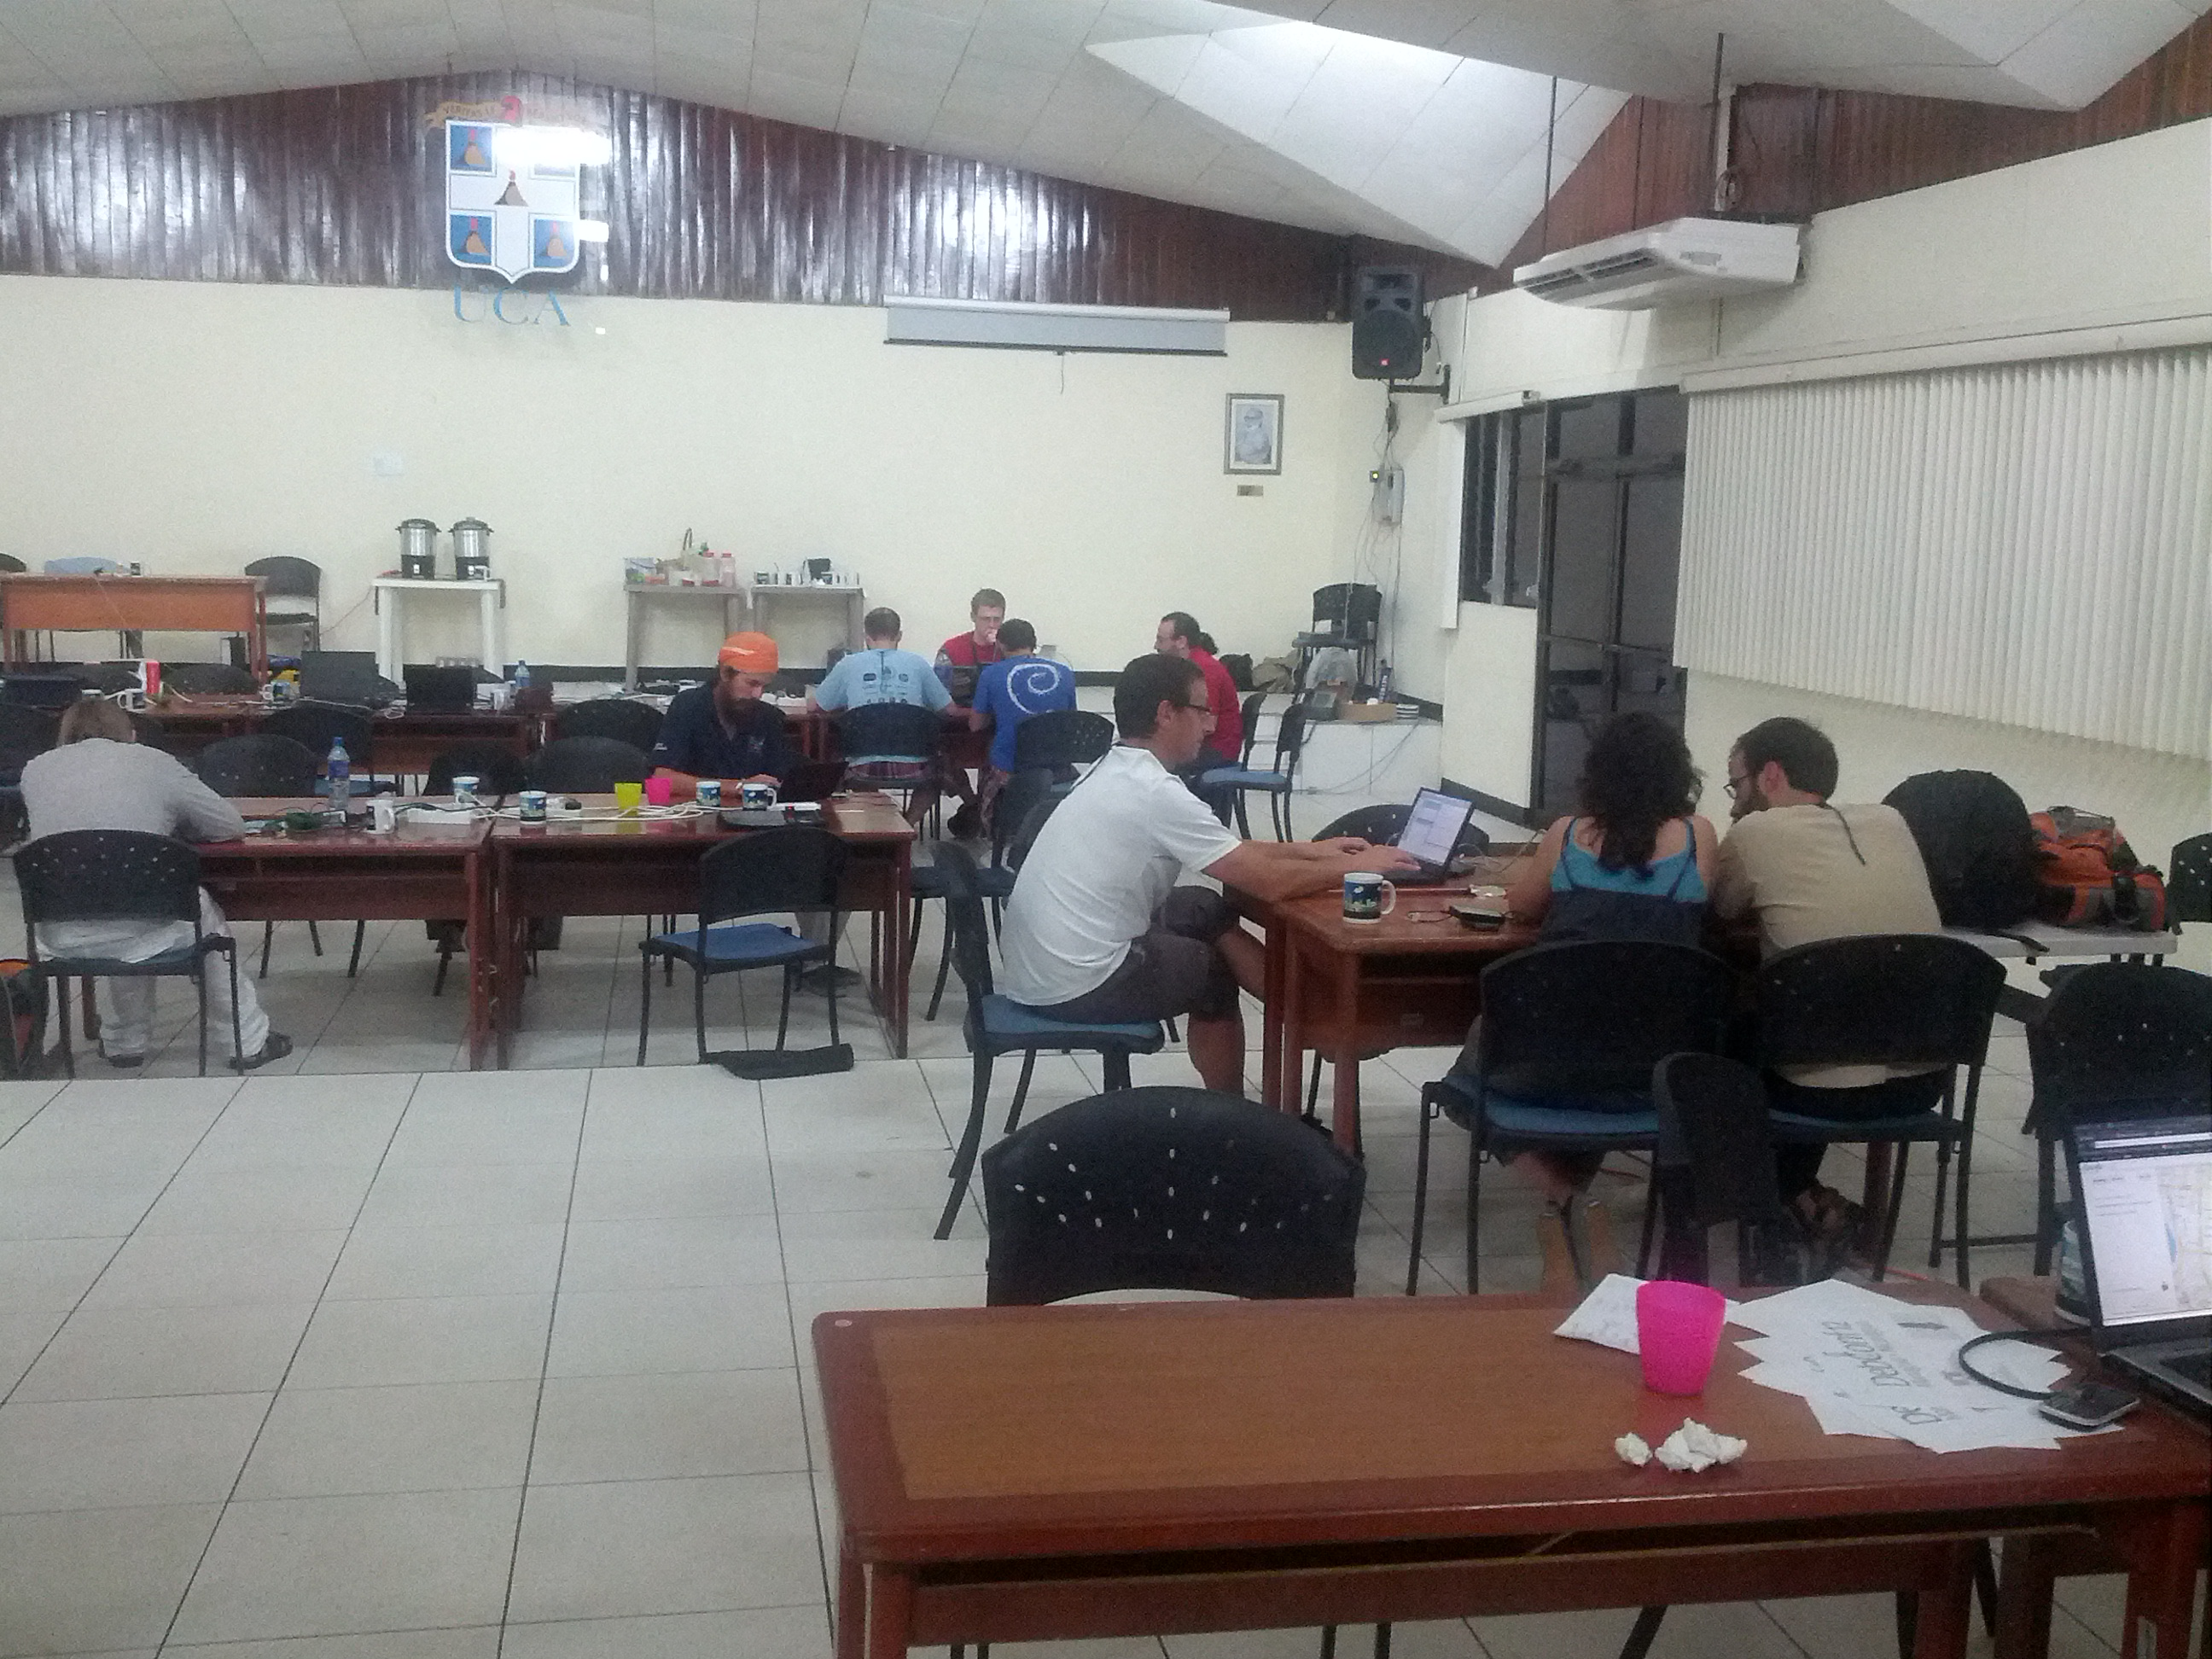
\includegraphics[width=0.8\hsize]{image201208/debconf12_hacklab02.jpg}
	\end{minipage}

 \item 食堂: 食堂は外にテントを張って、そこで食事しました。\\
	\begin{minipage}{0.4\hsize}
	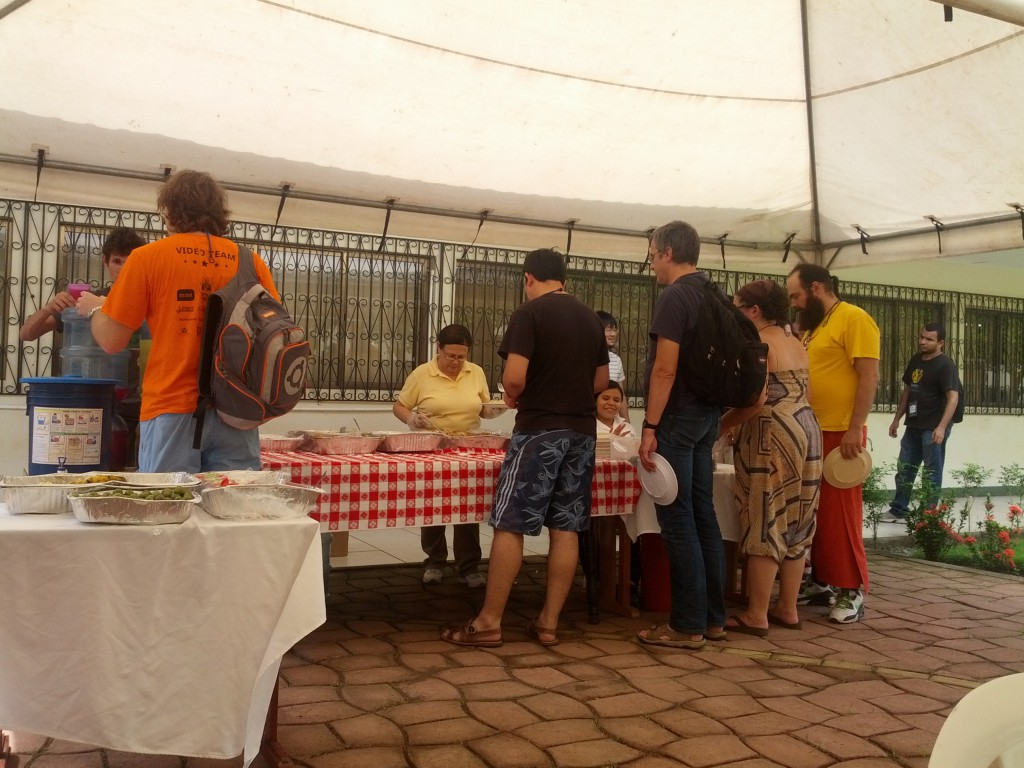
\includegraphics[width=0.8\hsize]{image201208/debconf12_diningroom01.jpg}
	\end{minipage}
	\begin{minipage}{0.4\hsize}
	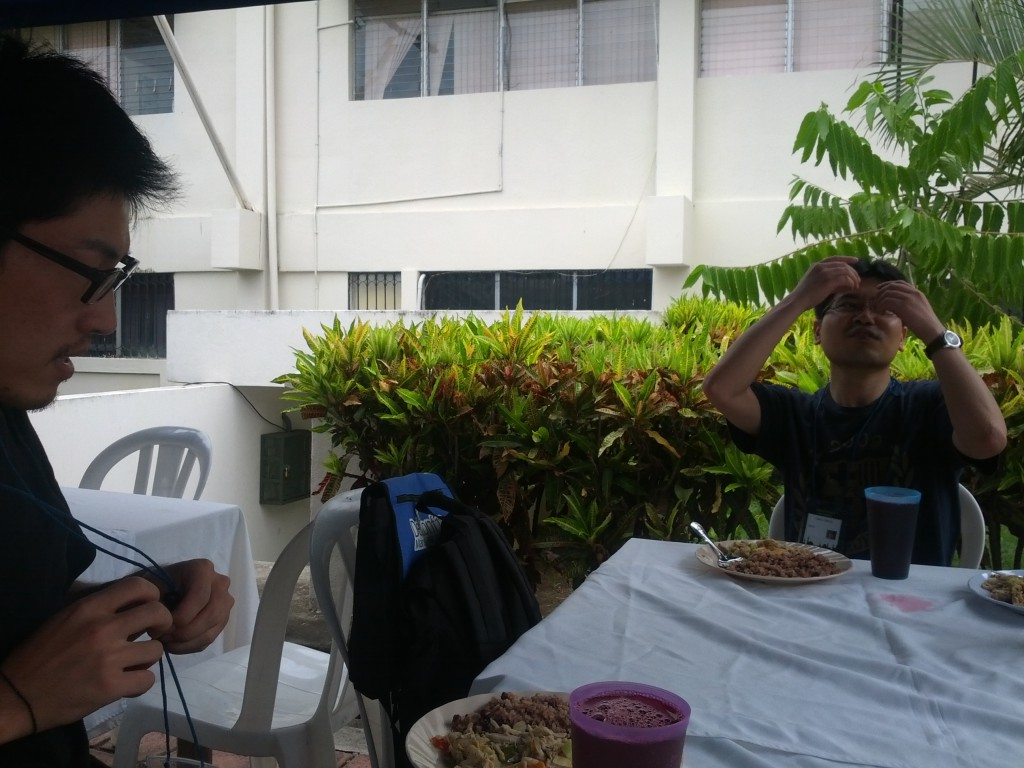
\includegraphics[width=0.8\hsize]{image201208/debconf12_diningroom02.jpg}
	\end{minipage}


 \item 宿泊したホテル:\\
	\begin{minipage}{0.4\hsize}
	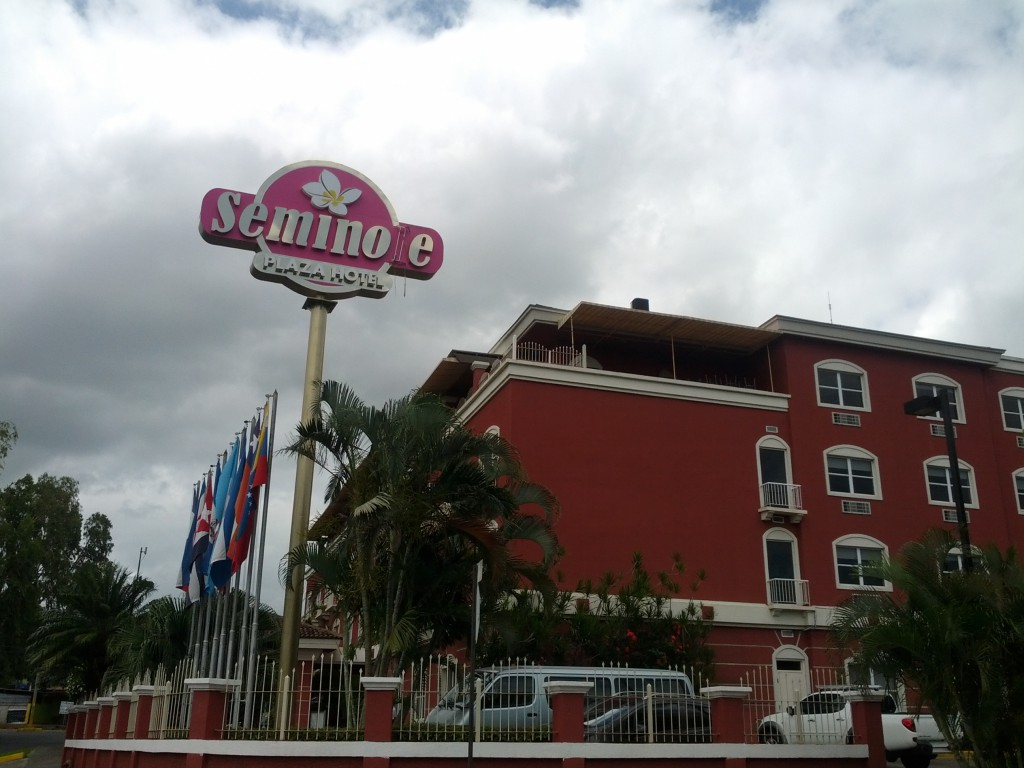
\includegraphics[width=0.8\hsize]{image201208/debconf12_hotel.jpg}
	\end{minipage}
        \begin{minipage}{0.4\hsize}
        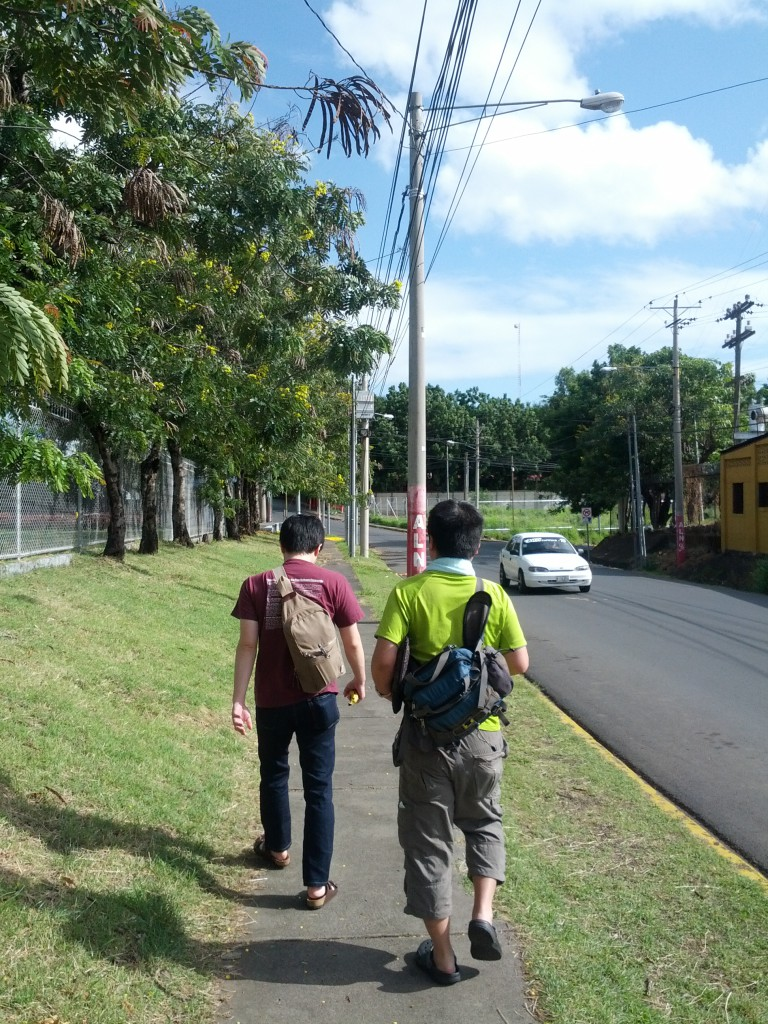
\includegraphics[width=0.8\hsize]{image201208/debconf12_hotel2.jpg}
        \end{minipage}

\end{itemize} 

\subsection{スケジュール}

7日のDebian Day で Debian Conference は開幕し、14日まで毎日いろいろな予
定が組まれていました。
11日だけはカンファレンス参加者で Day-trip を実施しました。

\subsection{主となった討論}

今回のDebconfは議論テーマを2日目は組み込み、4日目は
バーチャライゼーションなど、日によって分けられる方式が取られました。
また、地元からの参加者もわかるようにスペイン語での発表も多くありました。
個人的に今回のDebconfはあまり興味がある話題がなく、面白そうな話題があま
りなかったように感じました。その中でも私が参加した会議の内容からいくつか
取り上げて紹介します。

\subsubsection{Bits from the Release Team}

リリースチームによる次期リリースに関する発表が行われました。
今回のリリースから kibi(Cyril Brulebois)がリリースアシスタントに
加わることが発表されました。
また、Debconf開催前にフリーズが行われ、次のリリース内容についても発表がされ
ました。主要なソフトウェアを挙げると、KDEは4.8、GNOMEは3.4、Linux kernelは
3.2となります。RCバグ(当時で603個)が多く残っているため、バグつぶしに協力
して欲しいと報告が行われました。

\subsubsection{EFI BOF}
EFI(UEFI)についてのBOFが行われました。EFIのSecure boot に対応する
ためにはどのようにしたらいいのか、他のディストリビューションの対応
とDebian での対応方法について情報交換が行われました。
RedHat/Fedoraはブートローダと全てのカーネルスタックに署名する方法で対応
しているようです。またCanonical/Ubuntuはefilinuxのみに署名し対応する方法
を取っているとのこと。GPLv3の問題もありGrub2での対応は難しそうです。
今回のBOFでは良い案は出て来ませんでした。

\subsubsection{Multiarch crossbuilding}
Wookeyによる multiarch がサポートされた環境でのクロスビルドパッケージの
状況と問題点について発表が行われました。
現在 rebuildd と sbuild を使った クロスビルドファームを立ち上げ、クロス
ビルドテストを行なっていますが、まだいくつかの課題があるようです。
例えば multiarch のforeign
に対するクロスコンパイルに必要なパッケージの指定方法などに課題があります。
これを解決するためにパッケージのメタ情報として、cross-build-dep を指定し
これをaptで処理できるようにする機構を追加する(\#666772)といった方法があります。まだいくつか問題が残っているので協力して欲しいとのことでした。

\subsubsection{Build Debian with another compiler}
Sylvestre Ledru による LLVM を使ったDebianパッケージの全ビルドについて
の発表。現在、DebianのデフォルトのCコンパイラはGCCですが、LLVM/Clang 
を使ってみた結果と今後の予定について発表されました。
LLVMを使う理由として、ビルド速度が少しだけ速いということや、GCCより
より賢いコードパース機能が挙げられます。またGCCではない高性能な
コンパイラを選択できるということも良い点です。
Sylvestreは実験Debconf前に行われた LLVM 3.0 と3.1 の結果を元に
LLVMの利点を説明しました。
2012年の2月の時点でLLVM 3.0では、15658パッケージ中1381パッケージ 
(全体の8.8 \%)がビルドエラーになっているとのこと。
ほとんどのパッケージがビルドできているようです。
また 2012年の6月に行ったLLVM 3.1 では
17710 パッケージ中 2137パッケージ (全体の12.1 \%) がビルドに失敗している
ようです。この違いが出た理由は一部のオプションがサポートされていなかったり、
LLVM 3.0 では出なかったプログラムのバグ(プログラムミス)が検知できるよう
になったためです。
結果を\url{http://clang.debian.net/}から参照できます。
発表された時点では、まだGCCと切り替えできる機構が整備されていないため、
まだコンパイラ単体じゃないと利用できませんでした。今後は sbuild や dpkg
などのビルドツールにLLVM サポートを入れるように活動するとのこと。
商用コンパイラであるIntel コンパイラを使うためのツールやビルドも行なっている
ようなので、気になる方はSylvestreに連絡をとってみてください。
 
\subsubsection{ARM port(s) update}
ARMチームによる ARM ポーティングの状況について報告が行われました。
現在armelとarmhfの2つのアーキテクチャがあり前者は古いARM SoC(v4t)
を、後者は比較的新しいARM SoC(v7) をサポートしています。
armel はまだユーザもいるので今後もサポートしていく予定です。armhf は
次のリリースに含まれる予定ですが、動作させているマシンのメモリが1GB
しかないため、いくつかのソフトウェアがビルドできない等の問題が起きてい
るようです。この問題を解決するために ARM Server 向けのマシンをどこかから
(HPと交渉しているようだけど)借りて、Builddを置き換える予定みたいです。
この話の背景として、今後はモバイル端末だけでなく Server でもARMが使われる
ようになるため、それらをDebianでサポートするためのことも考えているとのこと。
その他、Raspbianや他のディストリビューションのサポート状況などについても
情報交換されました。

\subsubsection{AArch64 planning}
ARM 64bit サポートアーキテクチャである AArch64 サポートの
報告が行われました。AArch64 は ARMv7互換の64bit CPU ARMv8をサポート
するためのLinuxアーキテクチャ名です(LKMLでこの名前はどうなの?
と議論されていましたが)。まだCPUはまだ開発中で来年の頭に市場に投入される
と言われています。これを次のリリースである Jessie のサポートアーキテクチャ
にするためにARMチームは活動していると報告しました。
現在Linuxカーネル、ツールチェイン、dpkg、autoconf のサポートは完了して
おり、Qemuベースで動作しているとのこと。実際にそのデモも行われました。

\subsubsection{FreedomBox Update}
Bdale Garbee による FreedomBox の報告が行われました。
FreedomBox は Dreamplug などのARM Soc を使ったプラグ型サーバの
Linux ディストリビューションです。プライベートデータを
容易に扱うことのできるサーバを構築できることを目的としています。
今回、FreedomBoxを開発するための団体である FreedomBox Foundation の
紹介とFreedomBoxの成果をDebianにマージ完了の報告が行われました。
現在Dreamplugしかサポートしていませんが、今後他のマシンの対応もすると
のことです。

\subsection{Debconf14}
Debconf14 はマルティニーク(カリブ海の島。フランス領)、 
カナダのモントリオール、ベネズエラのプエルトラクルスが立候補しました。
マルティニークは飛行機でいくのが難しそうな国なのと十分なネットワーク
環境がないのでいまのところ難しそうです。モントリオールは設備がまだ不十分な
感じです。ベネズエラは既に国内のスポンサーも獲得しており、ホテルもいくつか
抑えてるとのこと。ネットワーク以外は網羅していると思いました。

\subsection{Daytrip}

\begin{minipage}{0.4\hsize}
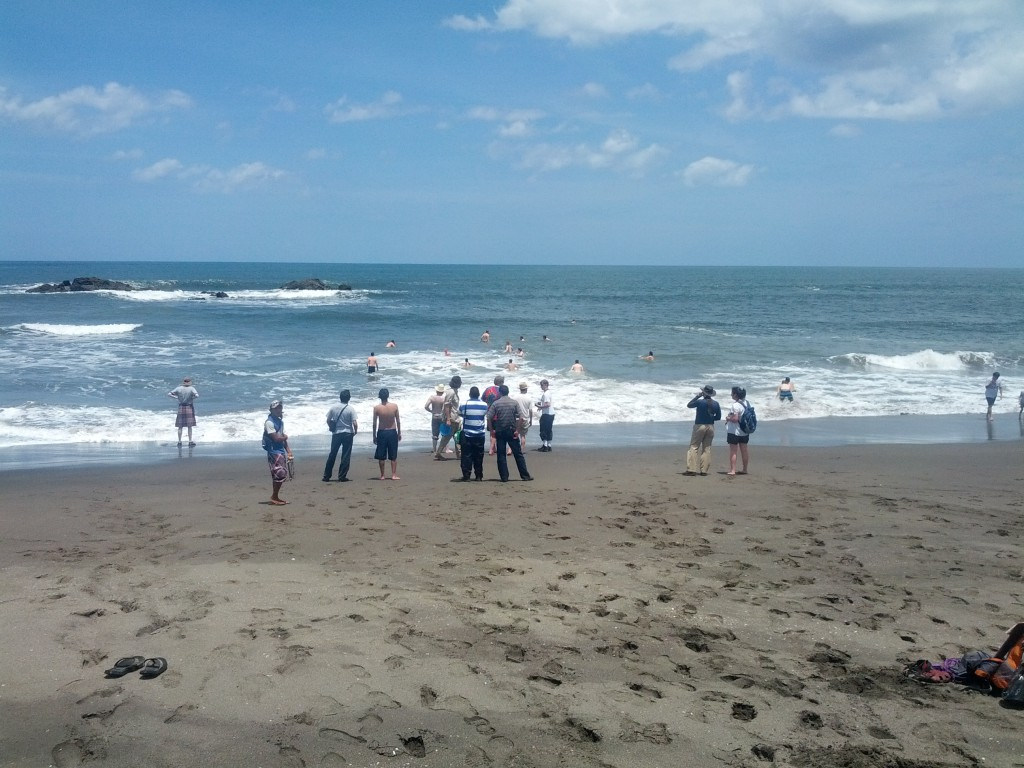
\includegraphics[width=0.8\hsize]{image201208/debconf12_daytrip01.jpg}
\end{minipage}
\begin{minipage}{0.4\hsize}
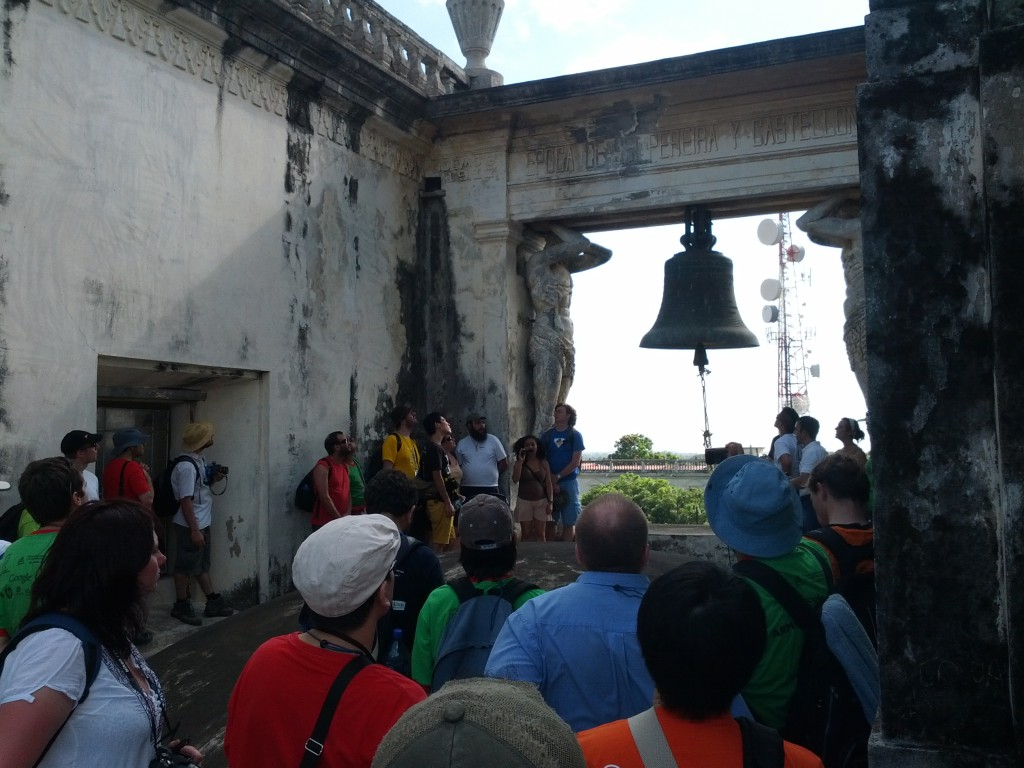
\includegraphics[width=0.8\hsize]{image201208/debconf12_daytrip03.jpg}
\end{minipage}

Debconf では一日、参加者で旅行をするというイベントがあります。今回の
Debconfでは レオン旧市街観光ツアー、火山観光ツアー、ジュアンベアノ島
観光ツアーのチームに別れ、Daytrip をしました。
矢吹以外の日本からの参加者は全員火山観光ツアーに登録しましたが、先日の
大雨の影響で火山ツアーは行く事ができず、海に行ったあとにレオン市街観光
を行いました。

\subsection{次回のDebconf}
次回のDebconf13はスイスのヴァーマルキュで開催される予定です。
日程は8月5日から18日です。キャンプ場を借りきってやるようですが、
周りに何もないように見えます。
ホテルという施設でもないのでシェラフ等を持っていく必要がありそうです。
普段とは異なったサバイバルになると思います。

\clearpage


%-------------------------------------------------------------------------------
\dancersection{月刊Debhelper}{野島 貴英}
%-------------------------------------------------------------------------------
\index{debhelper}
\subsection{今回のコマンド}

 debhelperのマニュアルを翻訳した際、いつか解析しようと思っていた以下のコマンド
2つを今回は取り上げます。

\begin{itemize}
\item dh\_makeshlibs
\item dh\_shlibdeps
\end{itemize}
\index{dh\_makeshlibs}
\index{dh\_shlibdeps}

 これらのdebhelperコマンドは、共有ライブラリとの依存関係をdebパッケージに
含める際に大変役立つコマンドとなります。

\subsection{予備知識}

 今回、共有ライブラリの知識、共有ライブラリのパッケージ作成に関する予備
知識、debパッケージの構造について、知識がある程度ある人向けに書いていま
す。基本的な事項は文献\cite{levine,sakai,satorutakabayashi,junichiuekawalibrary,man5deb}を参照すると参考になります。

\subsection{呼び出し方と動作}

 以下のように順に呼び出して利用します。

\begin{commandline}
$ dh_makeshlibs 
$ dh_shlibdeps
\end{commandline}

\subsubsection{dh\_makeshlibs}

 本コマンドの目的は、共有ライブラリのパッケージに特化した制御ファイルを生成するのが
目的となります。

このコマンドは呼び出されると以下の動作を行います。

\begin{description}
\item [Step 1.] パッケージ構築ディレクトリで作成した共有ライブラリを走査し、発見した共有ライブラリのSONAMEに記載されているバージョン番号と、ライブラリ名を、objdumpを使ってかき集めます。
\item [Step 2.] 得た情報を元に、パッケージ構築ディレクトリ以下のDEBIAN/shlibsファイルを作成します。
\item [Step 3.] パッケージ構築ディレクトリ以下のDEBIAN/postinst,DEBIAN/postrmを生成します。
\item [Step 4.] dpkg-gensymbolsコマンドを呼び出し、ソースパッケージにメンテナが含めたsymbolファイルを参考にしながら、更新したsymbolファイルを、パッケージ構築ディレクトリ以下のDEBIAN/symbolに作成します。
\end{description}

\subsubsection{dh\_shlibdeps}

 本コマンドの目的は、共有ライブラリの依存関係を算出して、後に制御ファイルとしてのcontrolファイルを生成する時に置換情報として使われる''debian/パッケージ名.substvars''ファイル(以下substvarsファイル)を更新します。

このコマンドは呼び出されると以下の動作を行います。

\begin{description}
\item [Step 1.] パッケージ構築ディレクトリで作成した、実行可能ファイル、共有ライブラリを探します。
\item [Step 2.] 見つけたファイルをdpkg-shlibdepsへ引き渡し、substvarsファイルを更新します。
\end{description}


\subsection{\$\{shlibs:Depends\}、 \$\{shlibs:Recommends\}マクロ}

 共有ライブラリとの依存関係を人手でメンテナンスしつづけるのは大変面倒な
作業になり、また、多くのケースでは機械的に依存関係を求める事も可能なので、
パッケージ作成時に機械的に共有ライブラリとの依存関係を生成出来る仕組みがあります。
こちらのマクロはこの機能を利用する為のものとなります。 dh\_shlibdepsは
debian/controlファイルの記述に含まれるこれらマクロを、算出した依存情報で書き換えてくれます。

  なお、手元のバイナリについてどんな内容で置き換えられるかは、
展開済みのソースパッケージの元で''dpkg-shlibdeps -O バイナリファイル''で検証できます。

\begin{commandline}
$ apt-get source gnome-shell
$ cd gnome-shell-3.0.2
$ dpkg-shlibdeps -O /usr/bin/gnome-shell
...SONAMEの形式にバージョン情報が無いものがある、まったく参照されていないライブラリがある等の警告が出る...
shlibs:Depends=gnome-bluetooth (>= 3.0.0), libatk1.0-0 (>= 1.12.4),
libc6 (>= 2.2.5), libcairo-gobject2 (>= 1.10.0), libcairo2 (>= 1.2.4),
libcanberra0 (>= 0.2), libclutter-1.0-0 (>= 1.10.0), libcogl-pango0
(>= 1.7.4), libcogl9 (>= 1.7.4), libcroco3 (>= 0.6.2), libdbus-1-3 (>=
1.0.2), libdbus-glib-1-2 (>= 0.78), libffi5 (>= 3.0.4), libfolks25 (>=
0.6.0), libgck-1-0 (>= 2.91.1), libgcr-3-1 (>= 2.91.1),
libgdk-pixbuf2.0-0 (>= 2.22.0), libgee2 (>= 0.5.0),
libgirepository-1.0-1 (>= 0.9.2), libgjs0-libmozjs185-1.0, libgjs0b
(>= 1.32.0), libgl1-mesa-glx | libgl1, libglib2.0-0 (>= 2.26.0),
libgnome-keyring0 (>= 2.20.3), libgnome-menu-3-0 (>= 3.2.0.1),
libgstreamer0.10-0 (>= 0.10.16), libgtk-3-0 (>= 3.0.0),
libjson-glib-1.0-0 (>= 0.12.0), libmozjs185-1.0 (>= 1.8.5-1.0.0+dfsg),
libmutter0 (>= 3.4), libmutter0 (<< 3.5), libnm-glib4 (>= 0.7.999),
libnm-util2 (>= 0.7.0), libnspr4 (>= 2:4.9-2~) | libnspr4-0d (>=
1.8.0.10), libp11-kit0 (>= 0.2), libpango1.0-0 (>= 1.14.0),
libpolkit-agent-1-0 (>= 0.94), libpolkit-gobject-1-0 (>= 0.94),
libpulse-mainloop-glib0 (>= 0.99.1), libpulse0 (>= 0.99.1),
libsoup2.4-1 (>= 2.4.0), libstartup-notification0 (>= 0.2),
libtelepathy-glib0 (>= 0.13.12), libtelepathy-logger2 (>= 0.2.0),
libx11-6, libxcomposite1 (>= 1:0.3-1), libxdamage1 (>= 1:1.1),
libxext6, libxfixes3, libxi6, libxml2 (>= 2.6.27)
\end{commandline}
% $
\subsection{shlibsファイルと、symbolファイル}
  
dh\_makeshlibsコマンドと、dh\_shlibdepsコマンドで重要な役割を持つ
ファイル2つについて説明します。

\subsubsection{shlibsファイル}

\begin{commandline}
ファイル形式:
[<type>: ]<library-name> <soname-version> <dependencies ...>

実例:
$ cat /var/lib/dpkg/info/libgtk2.0-0:amd64.shlibs
libgtk-x11-2.0 0 libgtk2.0-0 (>= 2.24.0)
libgdk-x11-2.0 0 libgtk2.0-0 (>= 2.24.0)
udeb: libgtk-x11-2.0 0 libgtk2.0-0-udeb (>= 2.24.0)
udeb: libgdk-x11-2.0 0 libgtk2.0-0-udeb (>= 2.24.0)
\end{commandline}
%$
 ライブラリのファイル名(library-name)と、SONAMEのバージョンの情報(soname-version)と、
パッケージの依存情報として記載すべき内容(dependencies)を記したファイルとなります。

 実例でいくと、「libgtk-x11-2.0は実際のライブラリの名前、SONAMEのバージョン番号は0、
パッケージの依存情報として記載すべき内容としては、''libgtk2.0-0 ($>=$ 2.24.0)''と記載
せよ」という意味になります。この場合、libgtk-x11-2.0.so.0をリンクしているバイナリ
(``objdump -p バイナリ''で、NEEDEDという文言で判定できます)のパッケージ依存情報
としては、''libgtk2.0-0 ($>=$ 2.24.0)''を記載しなさいという意味になります。

 dh\_makeshlibsコマンドで-Vオプションを使って明示的に指定しない限り、dependenciesの部分
はパッケージのバージョンで生成される為、最も単純で、最も保守的な共有ライブラリへの
依存関係情報となっているという特徴があります。

 shlibsファイルを使った依存関係算出の方法は最も基本的な方法ですので、
BUG\#634192、\#571776でdebian-policyへ掲載すべきとの要望があり、
対応がなされた模様です。こちらについては、     

\begin{commandline}
$ git clone 'http://anonscm.debian.org/git/dbnpolicy/policy.git'
\end{commandline}
%$

すればshlibsファイルに関する記載が大幅追記されたdebian policyが読めます。

\subsubsection{symbolファイル}

 共有ライブラリの提供している全シンボルと、各シンボルについて
搭載されたバージョンを記載したファイルを用意すると、shlibsファイルを使うよりも、
もっと柔軟で必要最小限の依存関係を算出出来るようになります。
こちらを実現しようとするものが、symbolファイルとなります。

\begin{commandline}
ファイル形式:
<soname> <main dependency template>
[| <alternative dependency template>]
[ as many alternative dependency templates as needed ]
    <symbol> <first-version>[ <id of dependency template>]
    [ as many symbols as needed ]

実例:
$ cat /var/lib/dpkg/info/libapr1.symbols
libapr-1.so.0 libapr1 #MINVER#
 apr__SHA256_Data@Base 1.2.7
 apr__SHA256_End@Base 1.2.7
 apr__SHA256_Final@Base 1.2.7
 ...中略...
 apr_global_mutex_lock@Base 1.2.7
 apr_global_mutex_lockfile@Base 1.4.2
 apr_global_mutex_name@Base 1.4.2
 apr_global_mutex_pool_get@Base 1.2.7
 ...中略...
\end{commandline}
%$

 こちらのsymbolファイルの実例ですと、SONAMEとして、libapr-1.so.0、
パッケージの依存情報として記載すべき内容は ``\verb!libapr1 #MINVER#!''
となります。なお、\verb!#MINVER#!は、dpkg-shlibdepsによって、
シンボルが過不足なく見つかる時のバージョンによって``\texttt{( $>=$ X.X.X)}''の形式で
置き換えられます。

 共有ライブラリの依存関係を洗い出す際、SONAMEの情報が変わらない限りは、
バイナリが必要としているシンボルのみを最小限搭載しているライブラリと、
シンボルがすべて見つかる最古のバージョンのみを依存関係として含めた方が、
パッケージの利用にあたって都合の良い事が多いです。ここで、

\begin{itemize}
\item バージョンの上がったライブラリの元でビルドして依存関係を求めたが、
実は古いバージョンのライブラリでも全く問題なく動的リンク出来る場合は
古いバージョンのライブラリも含んで依存対象としたい。
\item 依存しているライブラリAがライブラリBを必要としているが、
バイナリからはライブラリBのシンボルを一切利用していないので、
バイナリ本体の依存関係としてライブラリBを外したい
\end{itemize}

\begin{figure}[ht]
\begin{center}
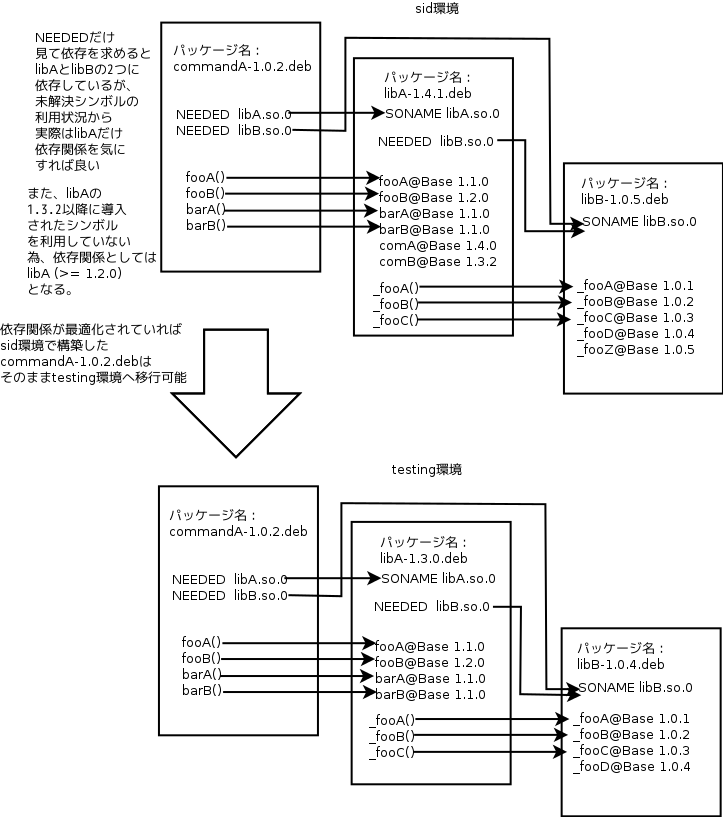
\includegraphics[width=12cm]{image201208/symbols-advantage.png}
\caption{\label{fig:symbol-deps}symbolファイルを利用した依存関係算出}
\end{center}
\end{figure}

という事を検討します。もし、こちらが出来ると、例えばsidからtesting
へバイナリパッケージを移動させるときに、依存関係にある数多くのライブラリ全部も同時に
sidからtestingへ完全に移動できるようになるまで、バイナリ本体をtestingの
ものとして移動出来ないという問題を極力避ける事ができます。\cite{hertzog}
(図\ref{fig:symbol-deps}参照)
    
\subsection{substvarsファイル}

 \$\{shlibs:Depends\}、\$\{shlibs:Recommends\}マクロなどのcontrolファイルに
含まれる情報を置き換える際にdebhelper共通で使われる中間ファイルとなります。
各debhelperコマンドがsubstvarsファイルに置き換えるべき内容を追記を繰り返すことにより、substvarsファイルは更新され、最後にdh\_gencontrolがマクロ部分をsubstvarsを参照しながら、適宜置き換えた制御ファイルとしてのcontrolファイルを生成します。

\subsection{内部で主に利用されているdpkgパッケージに含まれるコマンド}

 今回のdebhelperコマンドは内部でdpkgパッケージに含まれるいくつかのコマンド
を利用して処理を行っています。

\subsubsection{dpkg-gensymbols}

 dh\_makeshlibs内部にて、ライブラリメンテナがソースに含めているsymbolファイルを
元にし、実際に構築したライブラリから得られるシンボルの差分を含めたsymbolファイル
を生成するのに使われます。この生成されたsymbolファイルはライブラリ
パッケージのcontrolファイル群として含められます。

 dh\_makeshlibsの行うデフォルトの呼び出しでは、dpkg-gensymbolsは
ソースに含めているsymbolファイルからシンボルが廃止されたものがあることを
発見すると、DEBIAN/symbolファイルを一旦生成するものの、
エラーステータスを返却して終了してしまいます。この時、標準出力に違いを
diff形式で示します。もし、このような事が発生した場合は、メンテナはこのdiffを見ながら、
symbolファイルのメンテナンスを行う事になります。また、
生成されたsymbolファイルをメンテナは保管する事により、
次回のライブラリのバージョンアップに備える事になります。

\subsubsection{dpkg-shlibdeps}

 dh\_shlibdepsはほとんどdpkg-shlibdepsのラッパーコマンドとも
言えるぐらい、共有ライブラリの依存関係算出にあたって、
dpkg-shlibdepsをそのまま利用しています。

 dpkg-shlibdepsの動作は以下のとおりです。
\begin{description}
\item [Step 1.] コマンドラインから与えられたバイナリファイルが必要とする共有ライブラリへの
動的リンクに必要な情報を
\begin{commandline}
objdump -w -f -p -T -R バイナリファイル
\end{commandline}
コマンドを使って探ります。
\item [Step 2.] 得られた情報のうち、NEEDEDに記載されているSONAMEと同じファイル名を持つ
ライブラリファイルを\texttt{/lib},\texttt{/usr/lib}以下から探し当てます。
\item [Step 3.] 発見したライブラリファイルのフルパスを元にdpkg -Sを利用してライブラリの
パッケージ名を割り出します。
\item [Step 4.] ``\texttt{dpkg-query --control-path} ライブラリパッケージ名''を使って
\texttt{/var/lib/dpkg/info/}以下にあるライブラリパッケージの提供するshlibsファイル/
symbolファイルを取得します。
\item [Step 5.] Step 1.で得たバイナリファイルの動的リンクに必要なシンボル名と、
Step 4.で得たshlibsファイル/symbolファイルを検証することによりバイナリファイルにとって
最適な依存関係を算出します。
\item [Step 6.] substvarsファイルに算出した依存情報を記載します。
\end{description}

 参考: Step 5.の動作をどのように行っているかを観察するには、
\begin{commandline}
$ dpkg-shlibdeps -v -v -v -O バイナリファイル
\end{commandline}
%$
をバイナリファイルに対応するソースパッケージ展開後のディレクトリで、
実行するとよく判ります。

\subsubsection{おわりに}

 共有ライブラリの依存関係の対応すら2コマンドで担当出来るdebhelperコマンドと、
その心臓部を担うdpkgパッケージに含まれるコマンド群はよくできていると思いました。

\begin{thebibliography}{98}
\bibitem{levine} John R.Levine, 榊原 一矢/ポジティブエッジ 訳, ``Linkers \&
	 Loaders'', ISBN10 4274064379
\bibitem{sakai} 坂井 弘亮,  ``リンカ・ローダ実践開発テクニック'', ISBN10 4789838072
\bibitem{satorutakabayashi} 高林 哲ら, ``Binary Hacks'', ISBN10 4873112885
\bibitem{junichiuekawalibrary} Junichi Uekawa, ``Debian Library Packaging guide'',\url{http://www.netfort.gr.jp/~dancer/column/libpkg-guide/libpkg-guide.html}
\bibitem{man5deb} man 5 deb もしくはwikipediaのdeb(ファイルフォーマット),\url{http://ja.wikipedia.org/wiki/Deb_(%E3%83%95%E3%82%A1%E3%82%A4%E3%83%AB%E3%83%95%E3%82%A9%E3%83%BC%E3%83%9E%E3%83%83%E3%83%88)}

\bibitem{hertzog} 
Hertzog, ``Improved DpkgShlibdeps'', \url{http://wiki.debian.org/Projects/ImprovedDpkgShlibdeps}

\end{thebibliography}


%-------------------------------------------------------------------------------
\dancersection{ソフト開発以外の簡単Debian contribution(ドラフト版!)}{野島 貴英}
%-------------------------------------------------------------------------------
\index{かんたんなこんとりびゅーしょん@簡単なコントリビューション}
\subsection{はじめに}

 以前debconf11に参加した時、debconfの最後に行われるライトニング
トークで、「ソフト開発以外にDebianへ貢献するにはこんなのが
あるよ!」という発表がありました。この発表を聞いて以降、このあたりを
一度まとめてみたいなーと思っていました。

 ここでは、Debianをインストールしてちょっと慣れたぐらいの人がちょこちょこっと
Debianへ貢献する手段についてまとめてみます。きっと漏れもあると思うので、東京エリアDebian勉強会にてBOF形式で補完してみます。

\subsection{ソフト開発以外の簡単contribution作業一覧(ドラフト版!)}

\begin{itemize}
\item DDTSSの日本語訳をレビューしてみる、日本語に訳してみる。\\
(詳しくは「第53回東京エリアDebian勉強会資料」\url{http://tokyodebian.alioth.debian.org/pdf/debianmeetingresume200906.pdf}を参照ください。非常に良い解説とチュートリアルとなっています。)
\item BTSへBUG報告/何かの改善提案をしてみる。\\
(詳しくは「第43回 関西Debian勉強会資料」\url{http://wiki.debian.org/KansaiDebianMeeting/20110123}を参照ください。非常に良い解説とチュートリアルとなっています。)
\item \url{http://debtags.debian.net/edit/}でdebtagsをひたすら打ち込む。\\
(詳しくは「第63回東京エリアDebian勉強会資料」\url{http://tokyodebian.alioth.debian.org/pdf/debianmeetingresume201004.pdf}を参照ください。非常に良い解説とチュートリアルとなっています。)
\item \url{http://screenshots.debian.net/}へスクリーンショットを投稿しまくってみる。
\item \url{http://www.debianart.org/cchost/}へオリジナルの絵を送ってみる。
\item \url{debian-doc@debian.or.jp}にて投稿された翻訳のレビューをしてみる、未だ日本語に訳されていない文章を翻訳して投稿してみる。
\item \url{debian-users@debian.or.jp}にて投稿された質問に回答をしてみる。
\end{itemize}

\subsection{screenshots.debian.net}
\index{screenshots.debian.net}

 パッケージの動作のスクリーンショットを集めているサイトです。synapticパッケージマネージャ(aptitude install synapticで導入できます)にはプログラムの紹介の他に、プログラムが動作しているときのスクリーンショットを見る事ができます。このスクリーンショットのダウロード先がこのscreenshots.debian.netとなります。

 初めての方は以下のようにしてスクリーンショットを投稿できます。アカウント登録すら不要のお手軽サイトなので、面倒なユーザ登録も必要ありません。こちらに投稿され、無事審査をパスしたスクリーンショットは、世界中のDebianユーザが使っているsynapticパッケージマネージャで即閲覧できるようになります。

以下にスクリーンショットの投稿の仕方を記載します。

 \begin{description}
 \item [Step 1.] \url{http://screenshots.debian.net/packages/without_screenshots?search=&debtag=}をアクセスし、スクリーンショットが無いパッケージから適当なものを選びます。
 \item [Step 2.] 選んだパッケージを手元のDebianマシンへ導入します。
 \item [Step 3.] export LANG=Cを実行して、表示されるメッセージができるだけ英語になるようにしてプログラムを起動出来るようにします。
 \item [Step 4.] 導入したプログラムを起動します。
 \item [Step 5.] プログラムのスクリーンショットを撮ります。GNOME環境であれば、ALT+Print Screenでスクリーンショットを撮る事の出来るアプリケーションが起動します。
 \item [Step 6.] PNGファイルで撮ったスクリーンショットの画像を保存し、ImageMagickなどを使って画像サイズを最大でも800x600ぐらいにしてPNG形式で保存します。
 \item [Step 7.] \url{http://screenshots.debian.net/upload}をアクセスして、パッケージ名(Package name:)、パッケージのバージョン(Software version:)、どこの画面か等の説明(Screenshot description:)のフォームを半角英数字で埋め、ScrrenshotのChoose Fileを選んで、先ほど保存したスクリーンショット画像を選択します。
\item [Step 8.] 最後に[Upload screenshot]というボタンをクリックすると早速投稿が完了します。この時点では、サイト管理チームの審査が終ってないので、1日ぐらい待ちます。
\item [Step 9.] 無事審査がパスされると、\url{http://screenshots.debian.net/}の左上あたりの''Latest uploads...''という部分に、投稿したスクリーンショットが掲載されます。この時点で、synapticパッケージマネージャからもスクリーンショットが閲覧できるようになります。
\end{description}

やってみると判りますが、非常に簡単です。パッケージの魅力を伝えるのに、スクリーンショットの影響は少なくないと自分も考えています(特にゲームのパッケージ)。ぜひこの機会にスクリーンショットをあげまくってみてください。

 なお、注意事項として、撮影するスクリーンショットの元となるデータのライセンスには十分気をつけてください。これは大方のパッケージでは意識しなくても全く問題ないのですが、ゲーム等のパッケージのうちゲーム機/元々有料ソフトのエミュレータ環境等の、エミュレータのスクリーンショットでは、表示に使ったデータ次第では十分にライセンスが問題になり得ます。このあたりがちょっとでも心配な方は、ゲームのエミュレータ環境のスクリーンショットを投稿するのは、ライセンスに自信のある方以外は止めておいた方がよいでしょう。

\subsection{debianart.net}
\index{debianart.net}

 Debianに使われる様々なグラフィック/サウンドデータの投稿サイトとなります。直近では、wheezyの起動画面の背景画像、GNOME環境のデフォルトの背景画像などのコンテストが行われました。

 最近では、Debianプロジェクトにマスコットキャラクタが必要ということで、
マスコットキャラクタの図案の募集が行われていたようです。

 絵心のある方/写真撮影に興味のある方/サウンドアイコンに興味ある方で、我こそはという方はぜひ活用すると良いかもしれません。

 なお、Debianのプロジェクトである以上、投稿した絵/写真/音楽はいわゆるフリーなライセンスで扱われる事が出来るものに限ります。こちらはご注意ください。

\subsection{おわりに}

 Debianは多様性を重視するプロジェクトです。ソフト開発以外の貢献は大変重要で、協力者は日夜必要な状態です。やってみようという方は是非ご協力お願いします。

%-------------------------------------------------------------------------------
\dancersection{DebianでのC++11開発環境}{上川純一}
%-------------------------------------------------------------------------------
\index{c++11}
\subsection{はじめに}

2011年にながらくc++0xとして知られていた仕様が
C++11仕様\cite{n3242}として策定されC++言語機能が拡充されました。
そろそろC++11を使ったコードでも書いてみようかと思っている人もいるかもし
れません。
仕様が出てきてから一年以上たってもまだ仕様に完全に準拠したコンパイラというのは出てきてないようですが、
Debianに含まれているC++のコンパイラでもほとんどの機能は実装されてきています。
DebianでC++11を使ったコードを書くときにどういうパッケージをインストールしておくと便利なのか紹介します。

\subsection{サンプルコード}

とりあえずはC++11の機能を利用したサンプルコードを書いてみます。
auto と for ループを使ったものを試してみましょう。

\begin{commandline}
#include <iostream>
using namespace std;

int main(int argc, char **argv) {
  int hoge[] = { 1, 10, 12, 15};
  const char* fuga[] = { "hello", "world", "this is a", "message"};
  for (const auto& i : hoge) {
    cout << i << endl;
  }

  for (const auto& str : fuga) {
    cout << str << endl;
  }
  return 0;
}
\end{commandline}

\subsection{コンパイラー}

DebianでC++11準拠のソースコードをコンパイルできるコンパイラはGCCのG++とLLVMの
clang++ です。他にもあるかもしれませんが試していません。両方共すべての言語機能・ライブラリ関数
は実装していません\cite{gcc11support,clang11support}。実装していないので気になったところとしては \texttt{regex}, \texttt{attribute},
\verb!this_thead::sleep_for! などがあるようです。
とりあえずまずはインストールから。

\begin{commandline}
# apt-get install g++ clang
\end{commandline}

\subsubsection{GCC}
\index{g++}

g++ でコンパイルする場合は、--std=c++11 を指定してあげるとC++11モードでコンパイルします。

\begin{commandline}
$ g++ --std=c++11 auto.cc
$ ./a.out
\end{commandline}

\subsubsection{clang}
\index{clang}

Clangも同様で、C++11モードを指定してあげる必要があります。

\begin{commandline}
$ clang++ --std=c++11 auto.cc 
$ ./a.out
\end{commandline}

\subsection{ドキュメント}

\subsubsection{C++11 標準ライブラリ}

GCCもClangも両方共libstdc++ をライブラリとして利用しているようです。
libstdc++ のドキュメントは\texttt{libstdc++6-4.7-doc} パッケージにman
page形式で提供されています。
std namespaceにあるものはだいたい説明があるでしょう。
ただ、doxygenで自動生成されているからなのか若干クセがあります。
:: が \verb!_! に変換されていて、\verb!std::hogehoge!は\verb!std_hogehoge!という名前で登録されています。
他に混乱する例を挙げると、std::string は\verb!std_string!ではなく
\verb!std_basic_string! にドキュメントがあるのも最初はよくわかりませんでした。

\subsubsection{STL}

stl-manual パッケージにHTML形式でSTLのドキュメントが入っています。

\url{/usr/share/doc/stl-manual/html/index.html}

\subsubsection{GCC独自拡張についてのドキュメント}

gcc-doc パッケージにGCCでコマンドと言語仕様関連のInfoファイルがあります。

\subsubsection{その他のドキュメント}

その他これがあればいいだろうというドキュメントを紹介します。

C++でよく使うライブラリ、Boostのドキュメントは libboost1.49-doc パッケージにHTML形式ではいっています。

manpages-dev パッケージにLinuxのAPI関連のドキュメントがあります。

\subsection{最後に}

ひと通りC++11を利用するにあたって便利そうなものを紹介しました。もっと良い
物があるよというのがあればぜひ教えてください。

\begin{thebibliography}{98}
\bibitem{n3242} ``Working Draft, Standard for Programming Language
	C++'', 2011,
	\url{http://www.open-std.org/jtc1/sc22/wg21/docs/papers/2011/n3242.pdf}
\bibitem{bscxxfaq}
	Bjarne Stroustrup, C++ FAQ
	\url{http://www.stroustrup.com/C++11FAQ.html}
\bibitem{gcc11support}
	C++0x/C++11 Support in GCC, 
	\url{http://gcc.gnu.org/projects/cxx0x.html}

\bibitem{clang11support} 
	C++98 and C++11 Support in Clang, \url{http://clang.llvm.org/cxx_status.html}
\end{thebibliography}

% \printindex

\cleartooddpage

\vspace*{15cm}
\hrule
\vspace{2mm}

\includegraphics[width=2cm]{image200502/openlogo-nd.eps}
\noindent \Large \bf Debian 勉強会資料\\
\noindent \normalfont \debmtgyear{}年\debmtgmonth{}月\debmtgdate{}日 \hspace{5mm}  初版第1刷発行\\
\noindent \normalfont 東京エリア Debian 勉強会 (編集・印刷・発行)\\
\hrule

\end{document}
